\section{Phân tích và mô tả yêu cầu dữ liệu}
\subsection{Tìm hiểu ứng dụng hoặc hệ thống liên quan}
%TODO
Tên hệ thống: \textbf{CodeLearn} - Nền tảng học tập trực tuyến.

Đường dẫn: \url{https://codelearn.io}

Phân tích nghiệp vụ chính của hệ thống: Hệ thống CodeLearn vận hành với nhiều nghiệp vụ chính. Trước hết, người dùng có thể đăng ký tài khoản bằng email hoặc mạng xã hội, sau đó truy cập hồ sơ cá nhân để theo dõi lịch sử học tập và tiến độ từng khóa học. Mỗi khóa học bao gồm nhiều chương và bài học, có thể ở dạng lý thuyết, video hoặc bài tập lập trình trực tiếp trên trình duyệt. Hệ thống tự động chấm điểm các bài tập dựa trên bộ test công khai và ẩn, trả về kết quả chi tiết về độ chính xác, thời gian và bộ nhớ sử dụng. Khi hoàn thành tối thiểu 80\% nội dung và đạt điểm chuẩn, học viên được cấp chứng chỉ điện tử và có thể để lại đánh giá, nhận xét khóa học. Bên cạnh đó, hệ thống hỗ trợ diễn đàn hỏi đáp, nơi học viên và giảng viên cùng trao đổi kiến thức. Ngoài học tập, CodeLearn còn tổ chức các cuộc thi lập trình trực tuyến với xếp hạng tự động theo điểm và thời gian. Một số khóa học nâng cao yêu cầu thanh toán, có hỗ trợ mã giảm giá và chính sách hoàn tiền. Cuối cùng, mô-đun quản trị cho phép giảng viên và quản trị viên quản lý nội dung, người dùng, bài tập và thống kê hoạt động toàn hệ thống.

\begin{figure}[!htp]
    \centering
    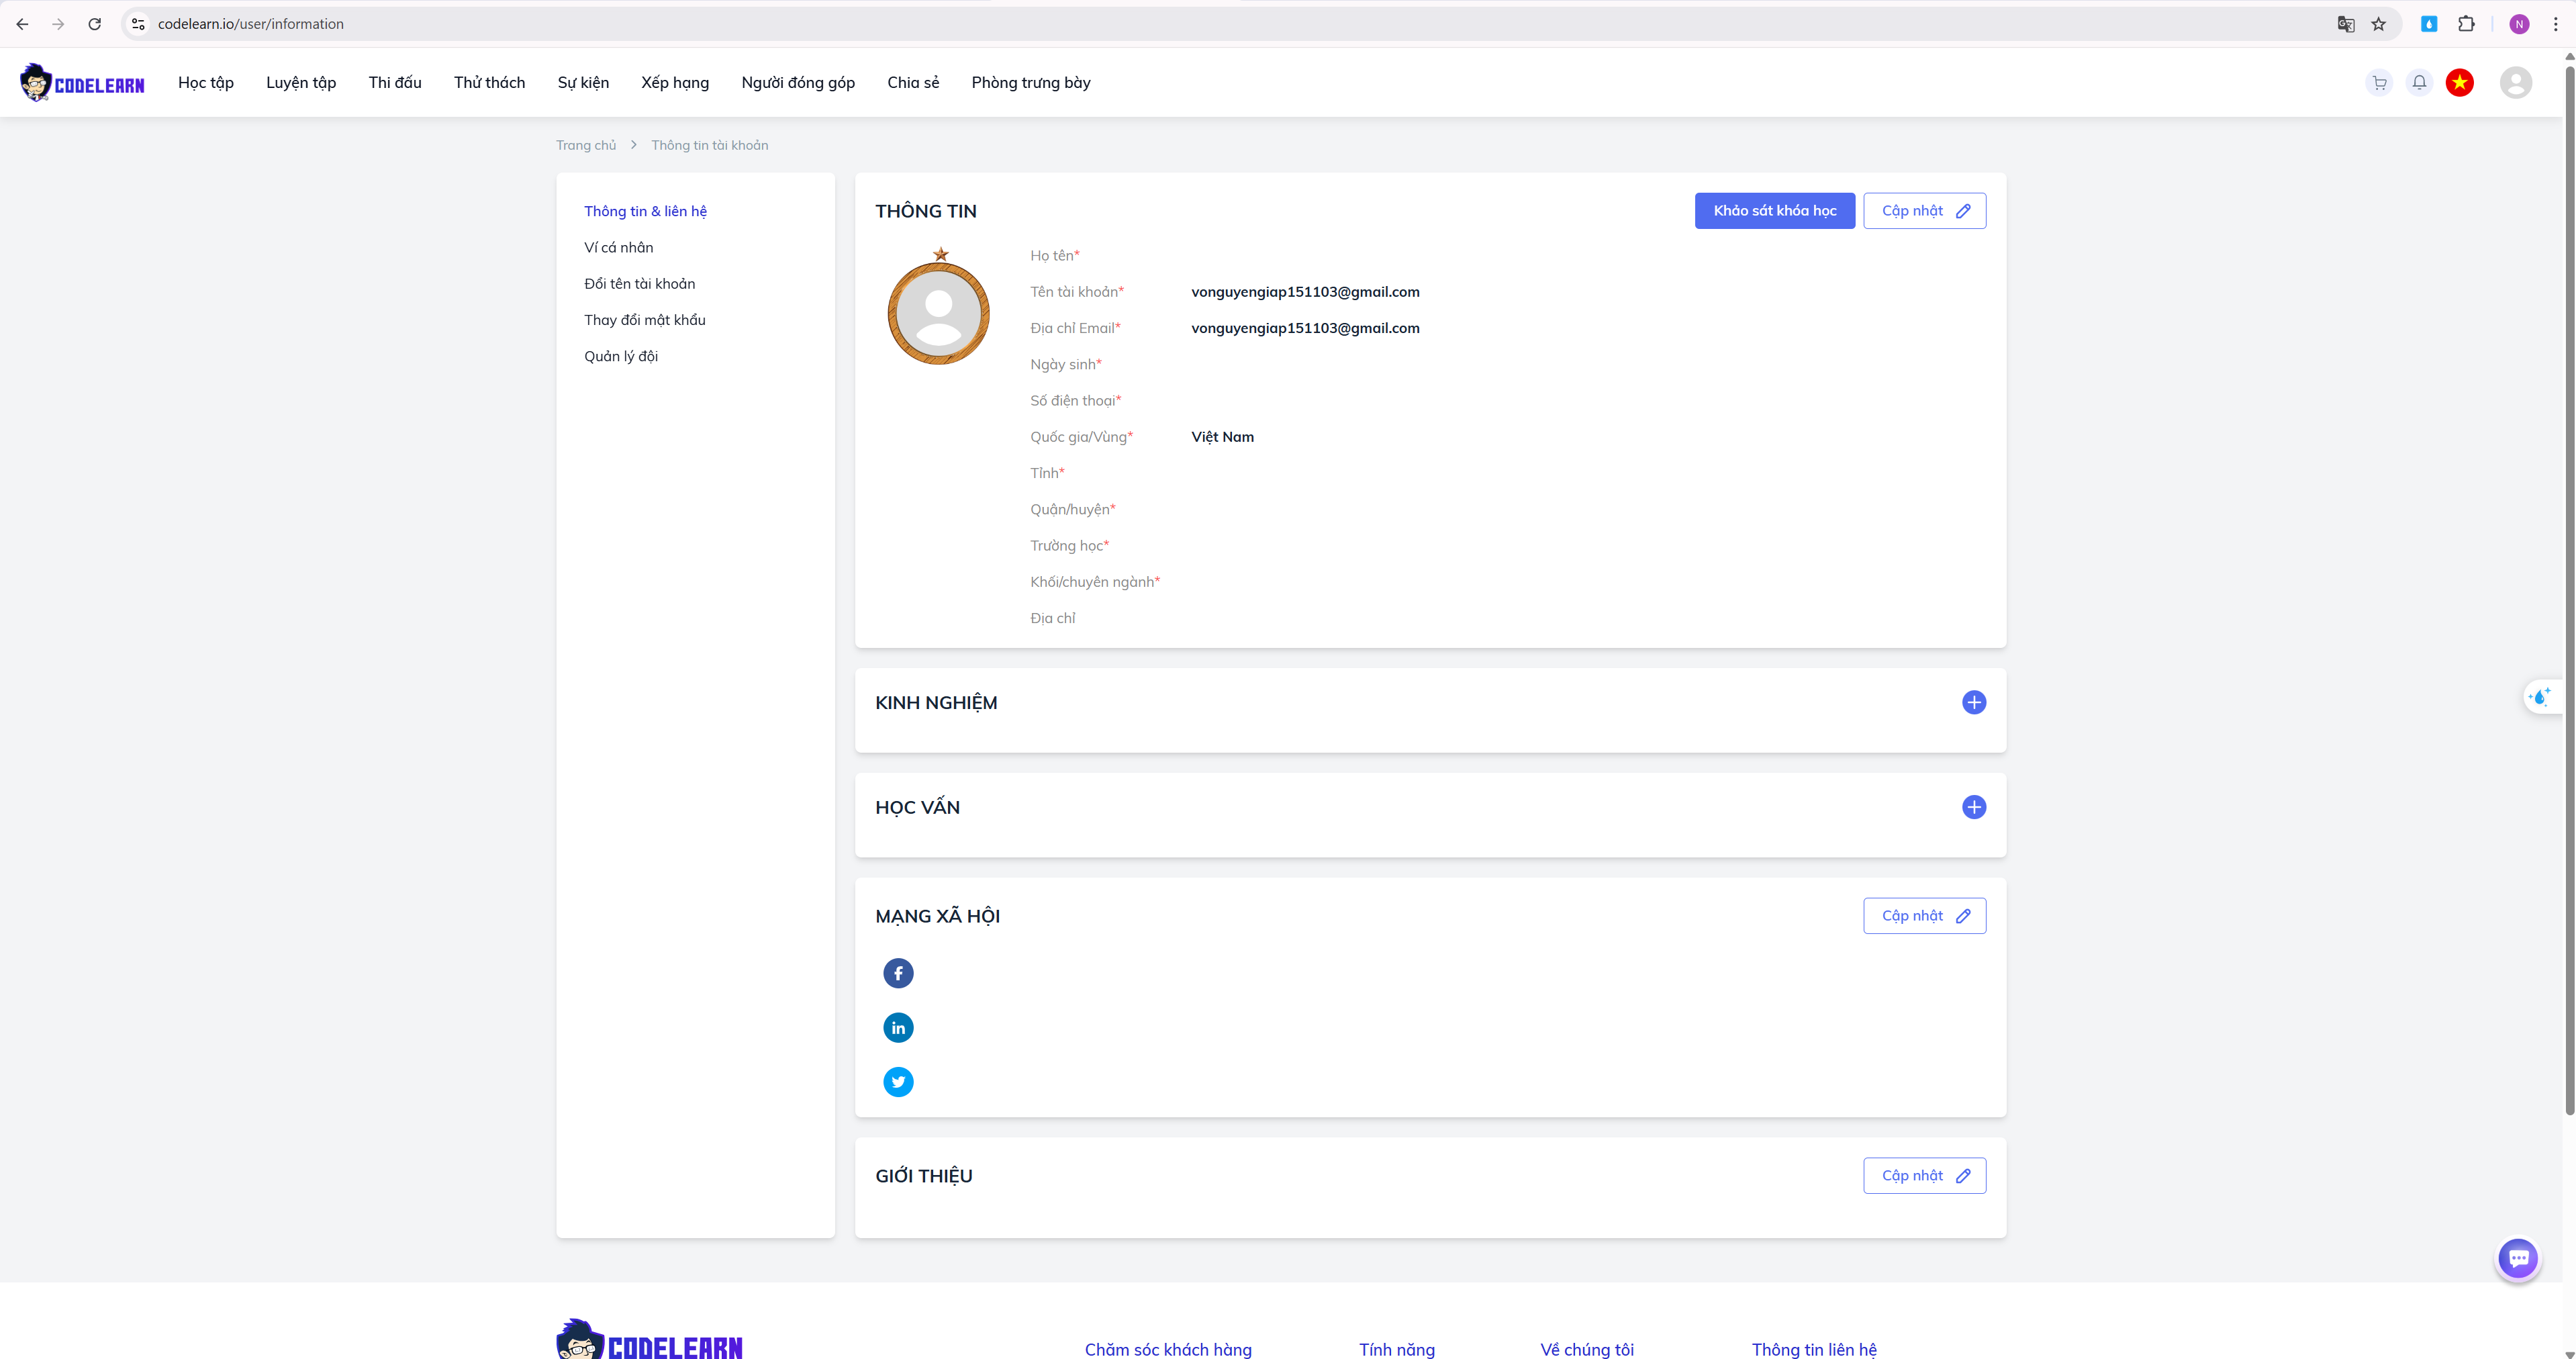
\includegraphics[width=1\linewidth]{picture/minh_chung_1.png}
    \caption{Thông tin của người đăng ký}
\end{figure}

\begin{figure}[!htp]
    \centering
    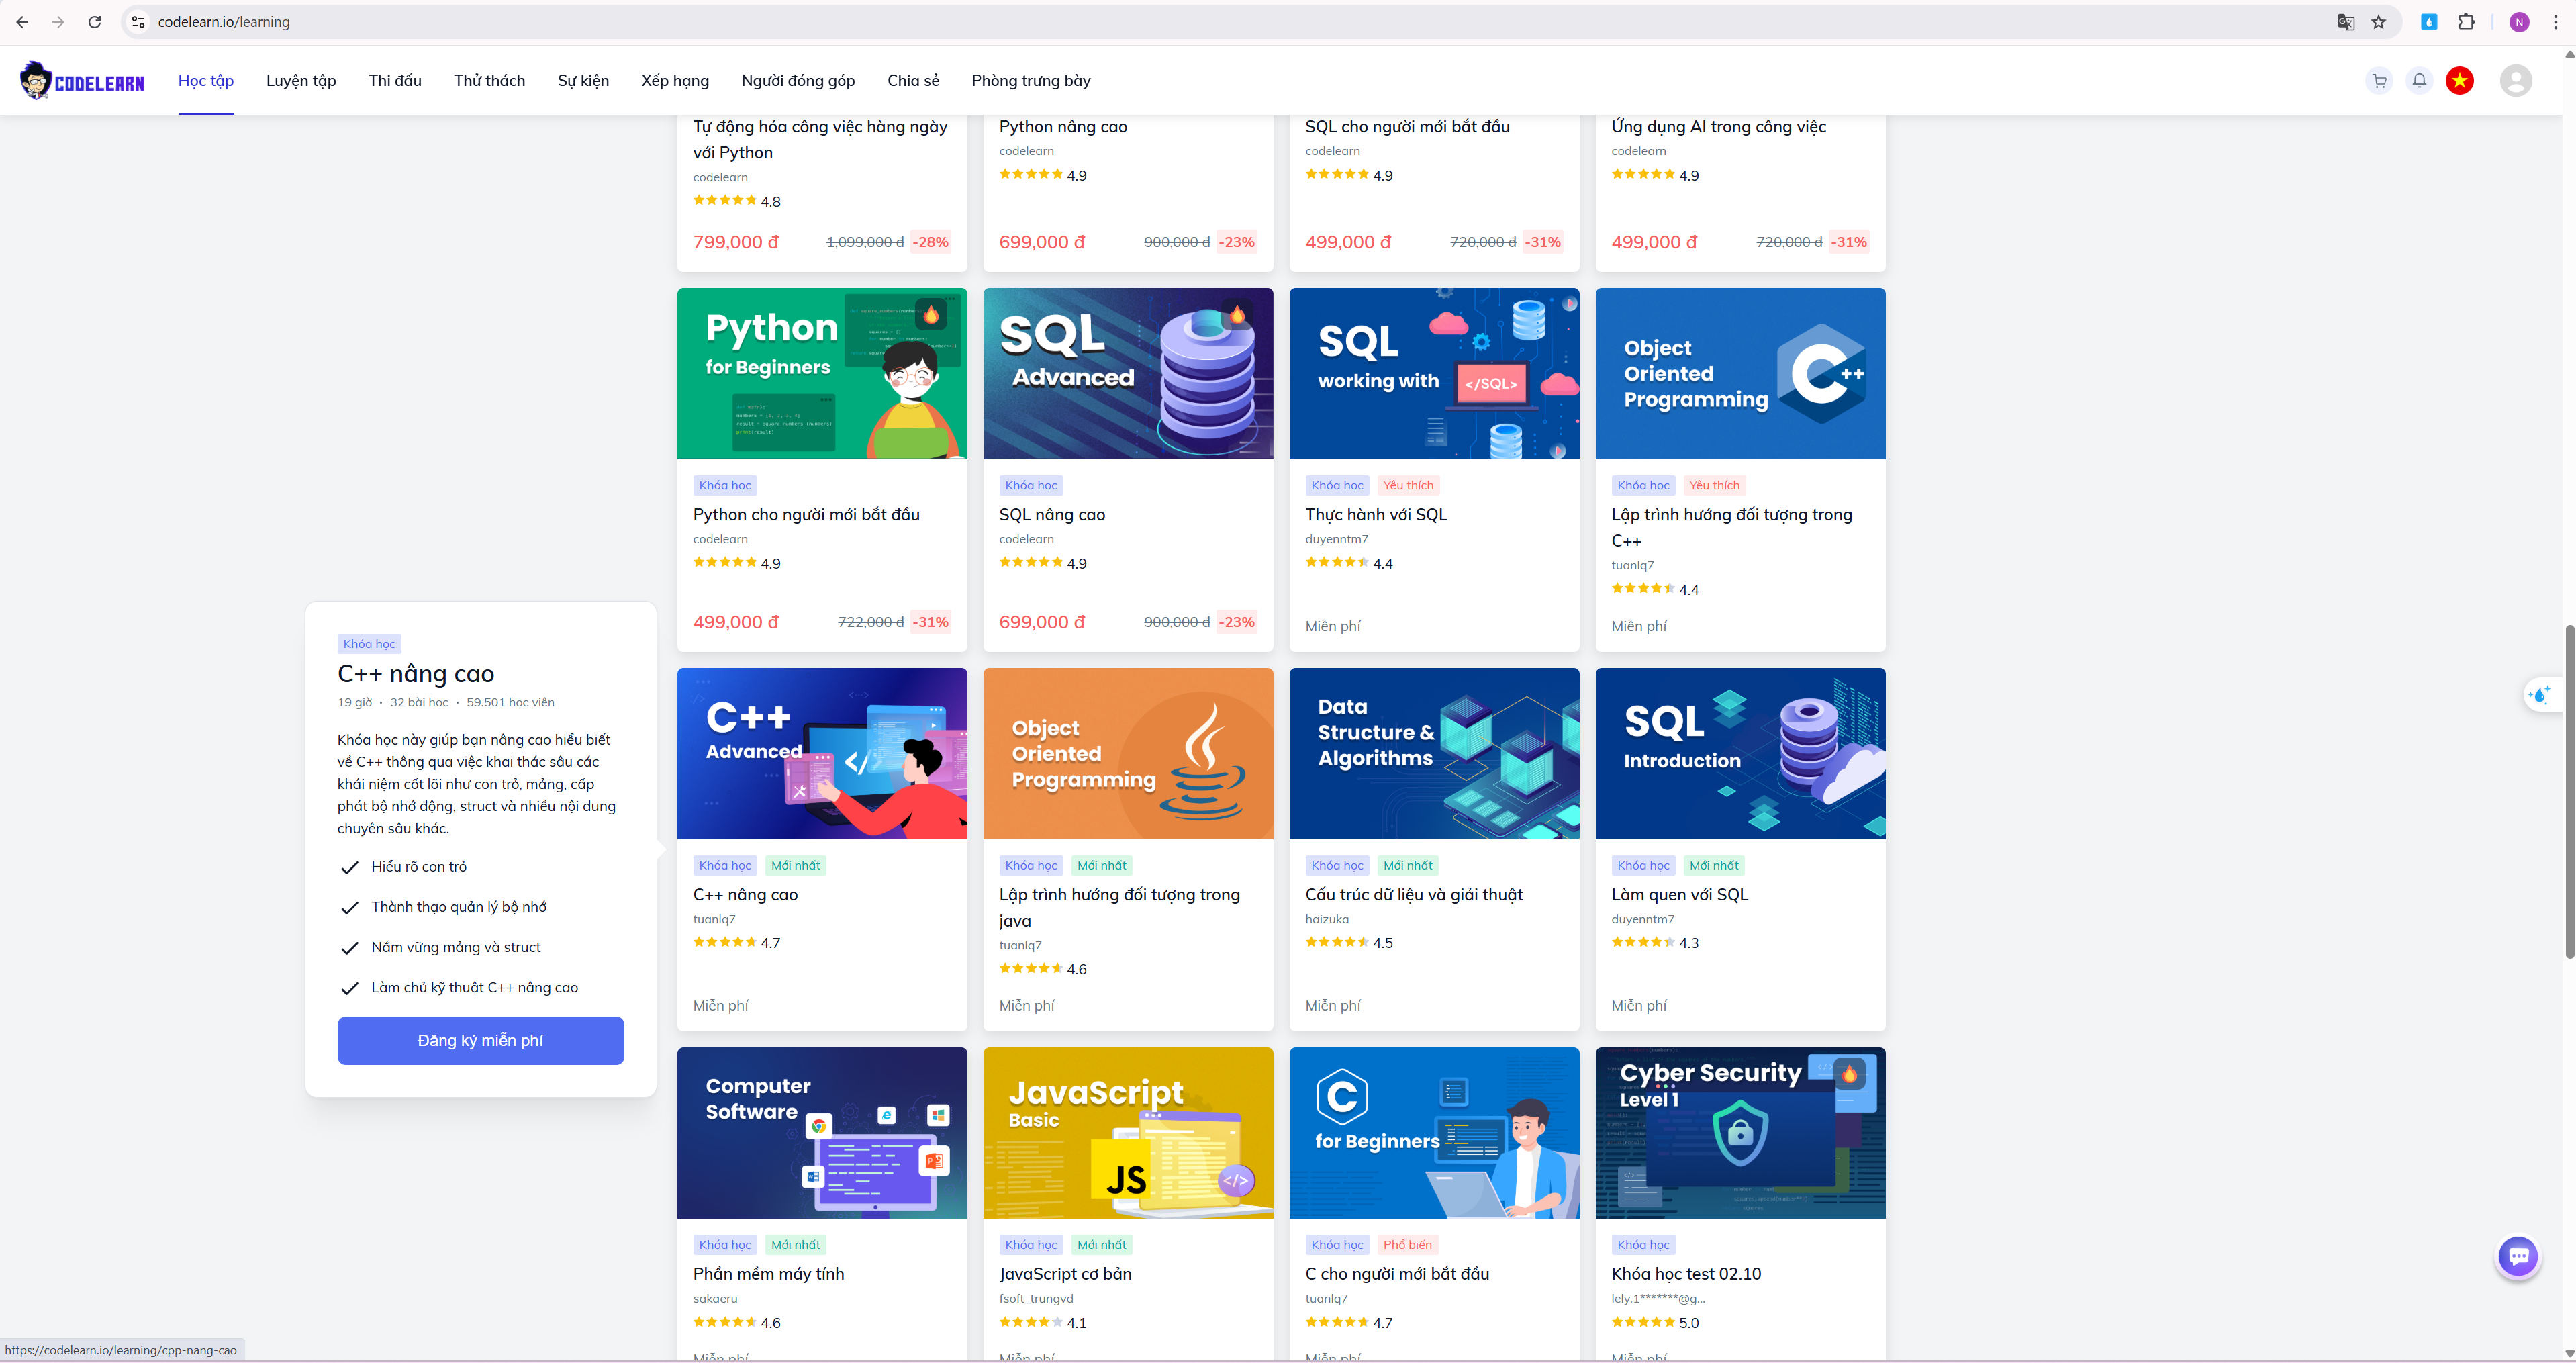
\includegraphics[width=1\linewidth]{picture/minh_chung_2.png}
    \caption{Thông tin về các khóa học}
\end{figure}

\begin{figure}[!htp]
    \centering
    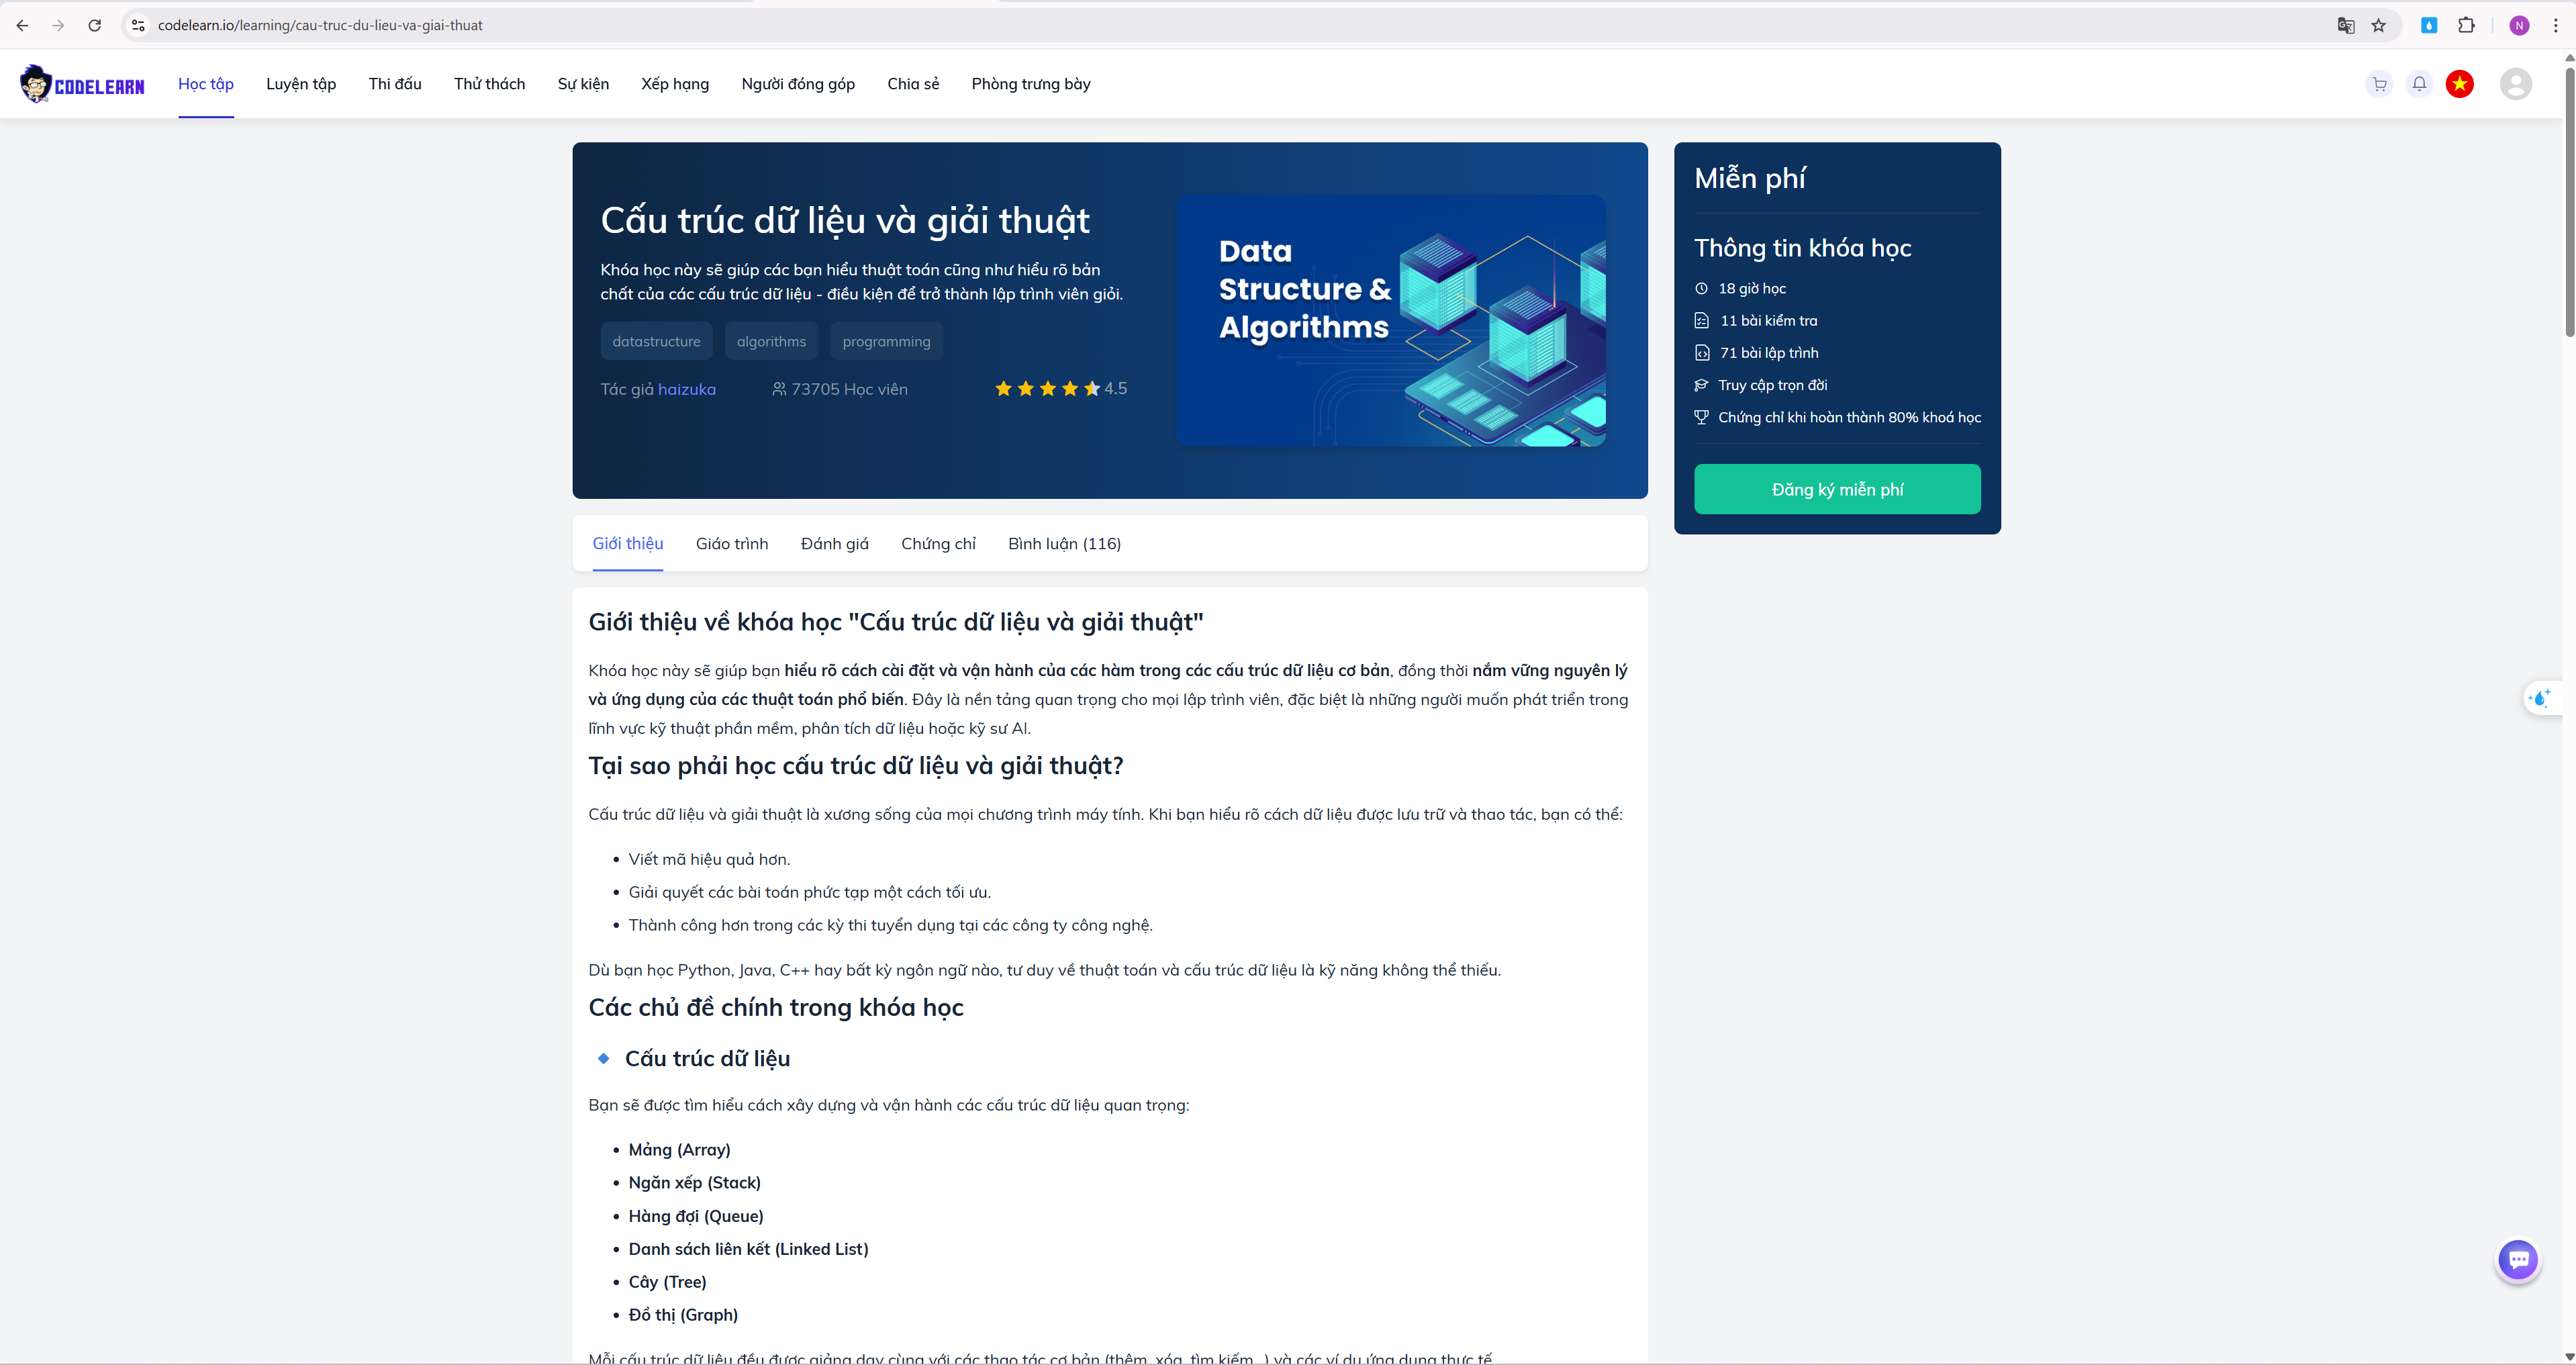
\includegraphics[width=1\linewidth]{picture/minh_chung_3.png}
    \caption{Thông tin chi tiết một khoá học}
\end{figure}

\begin{figure}[!htp]
    \centering
    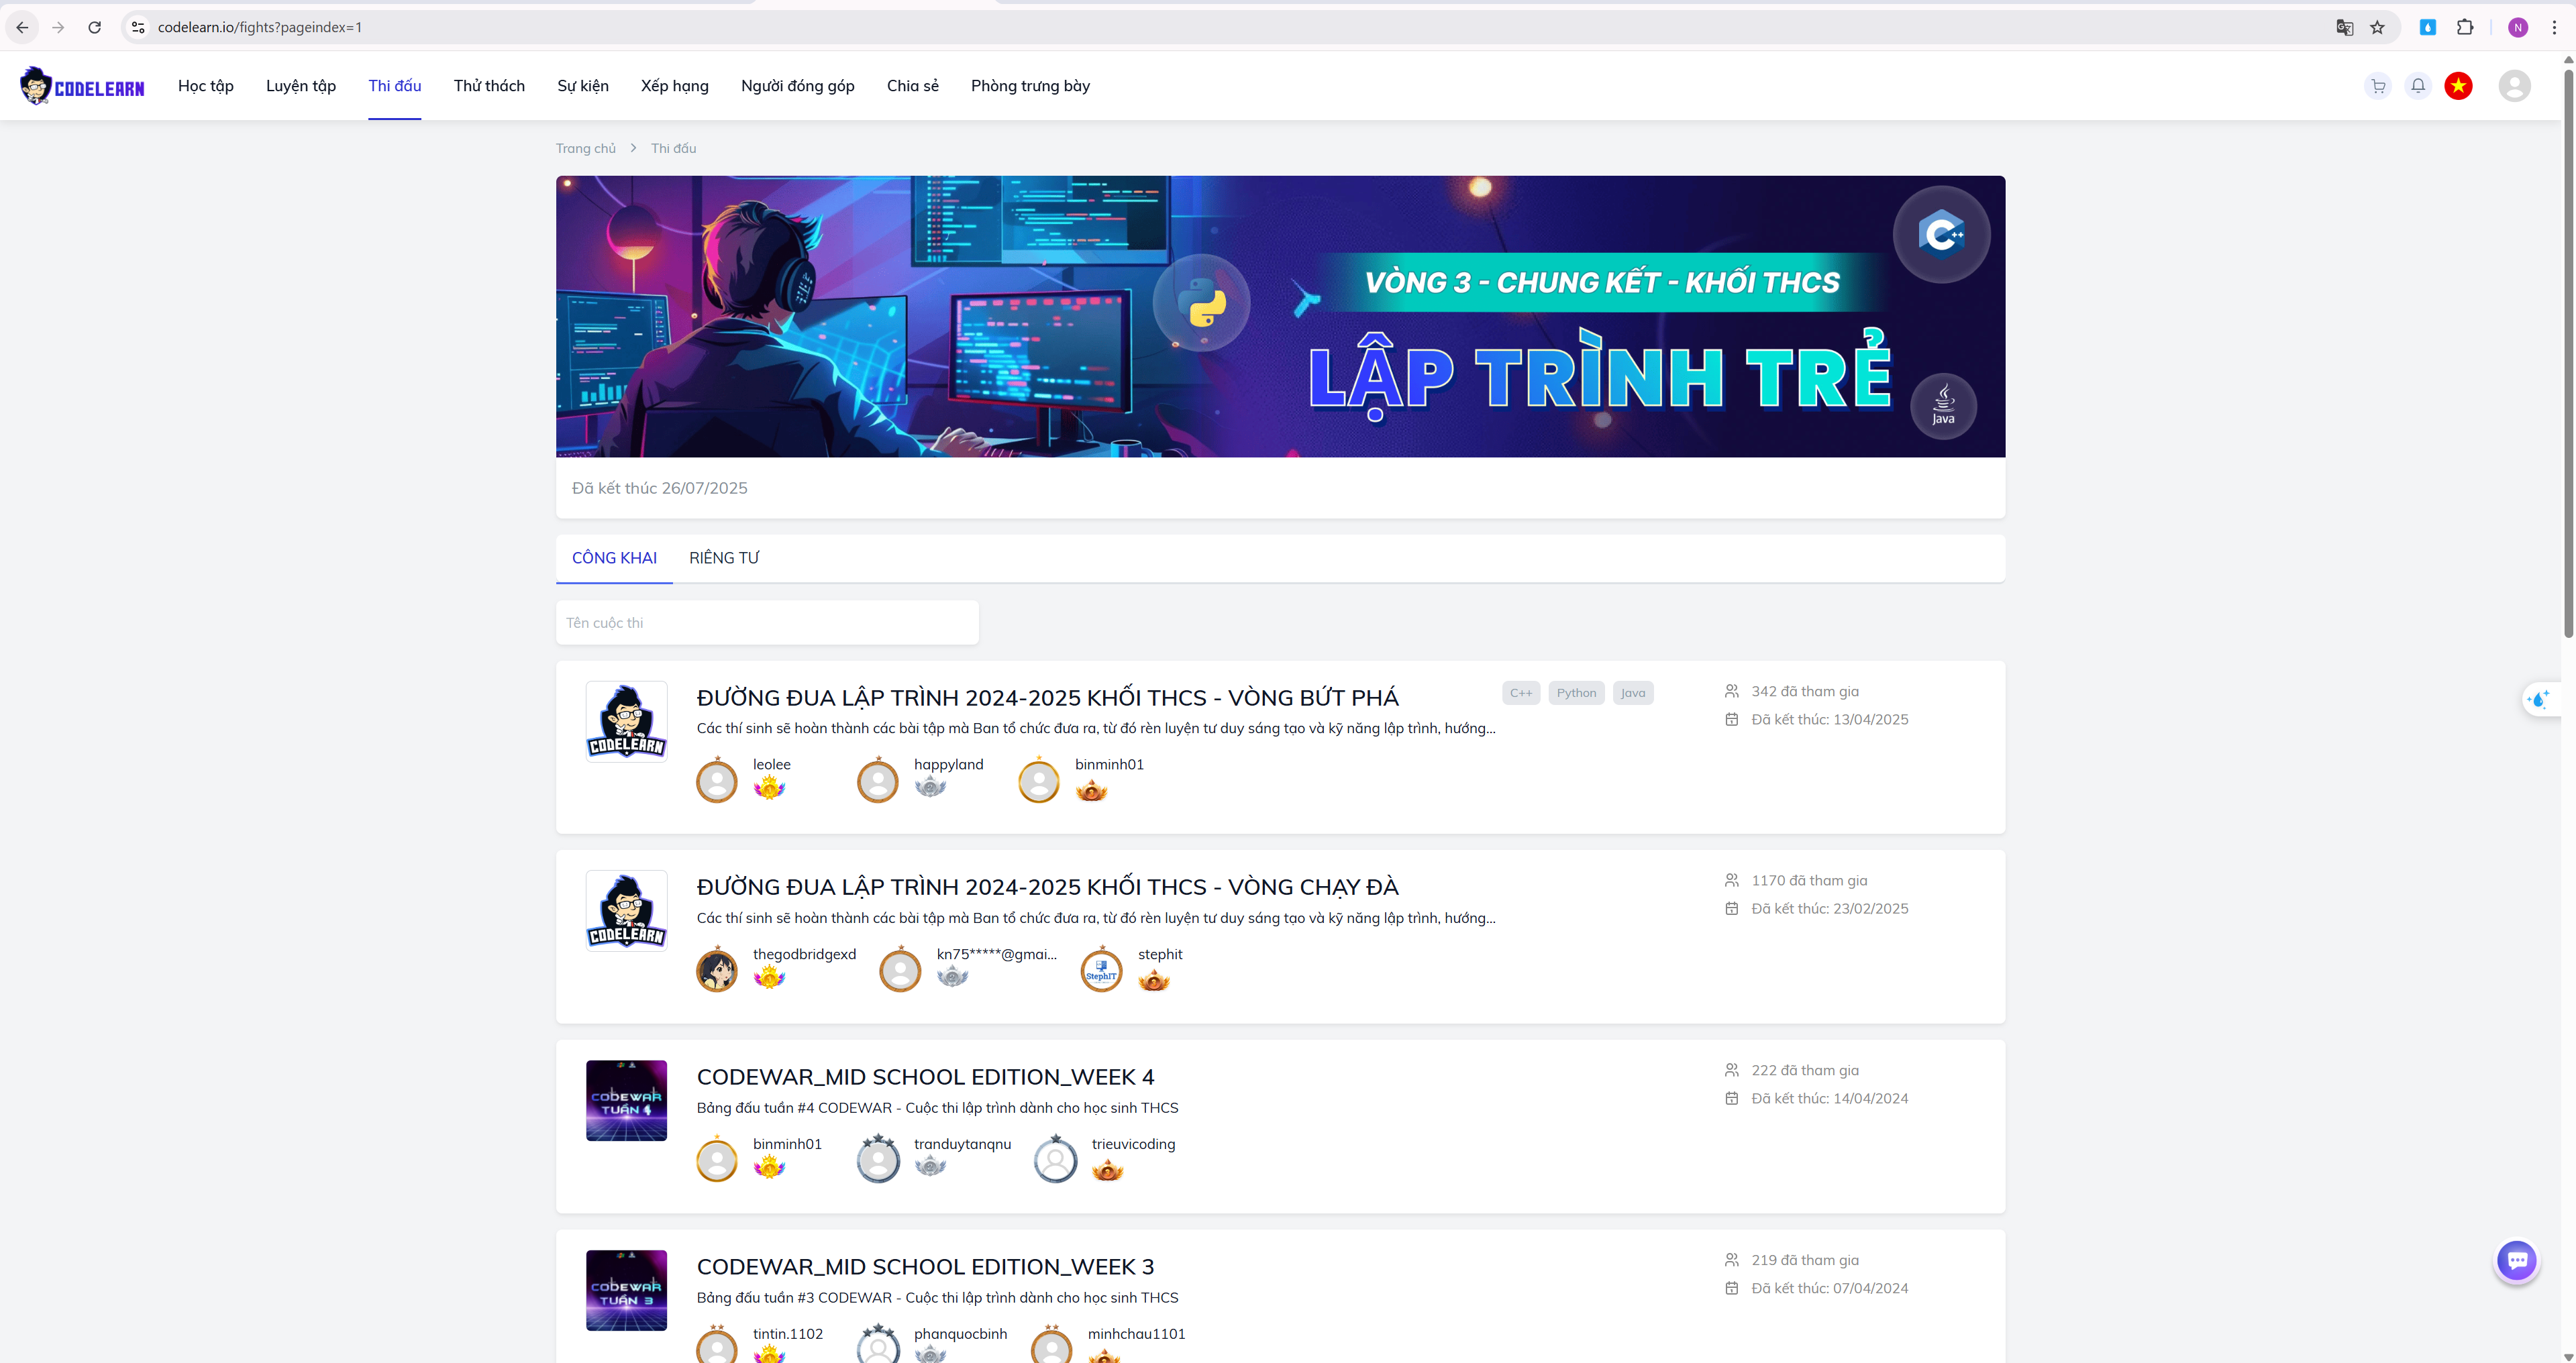
\includegraphics[width=1\linewidth]{picture/minh_chung_4.png}
    \caption{Thông tin về các cuộc thi}
\end{figure}

\begin{figure}
    \centering
    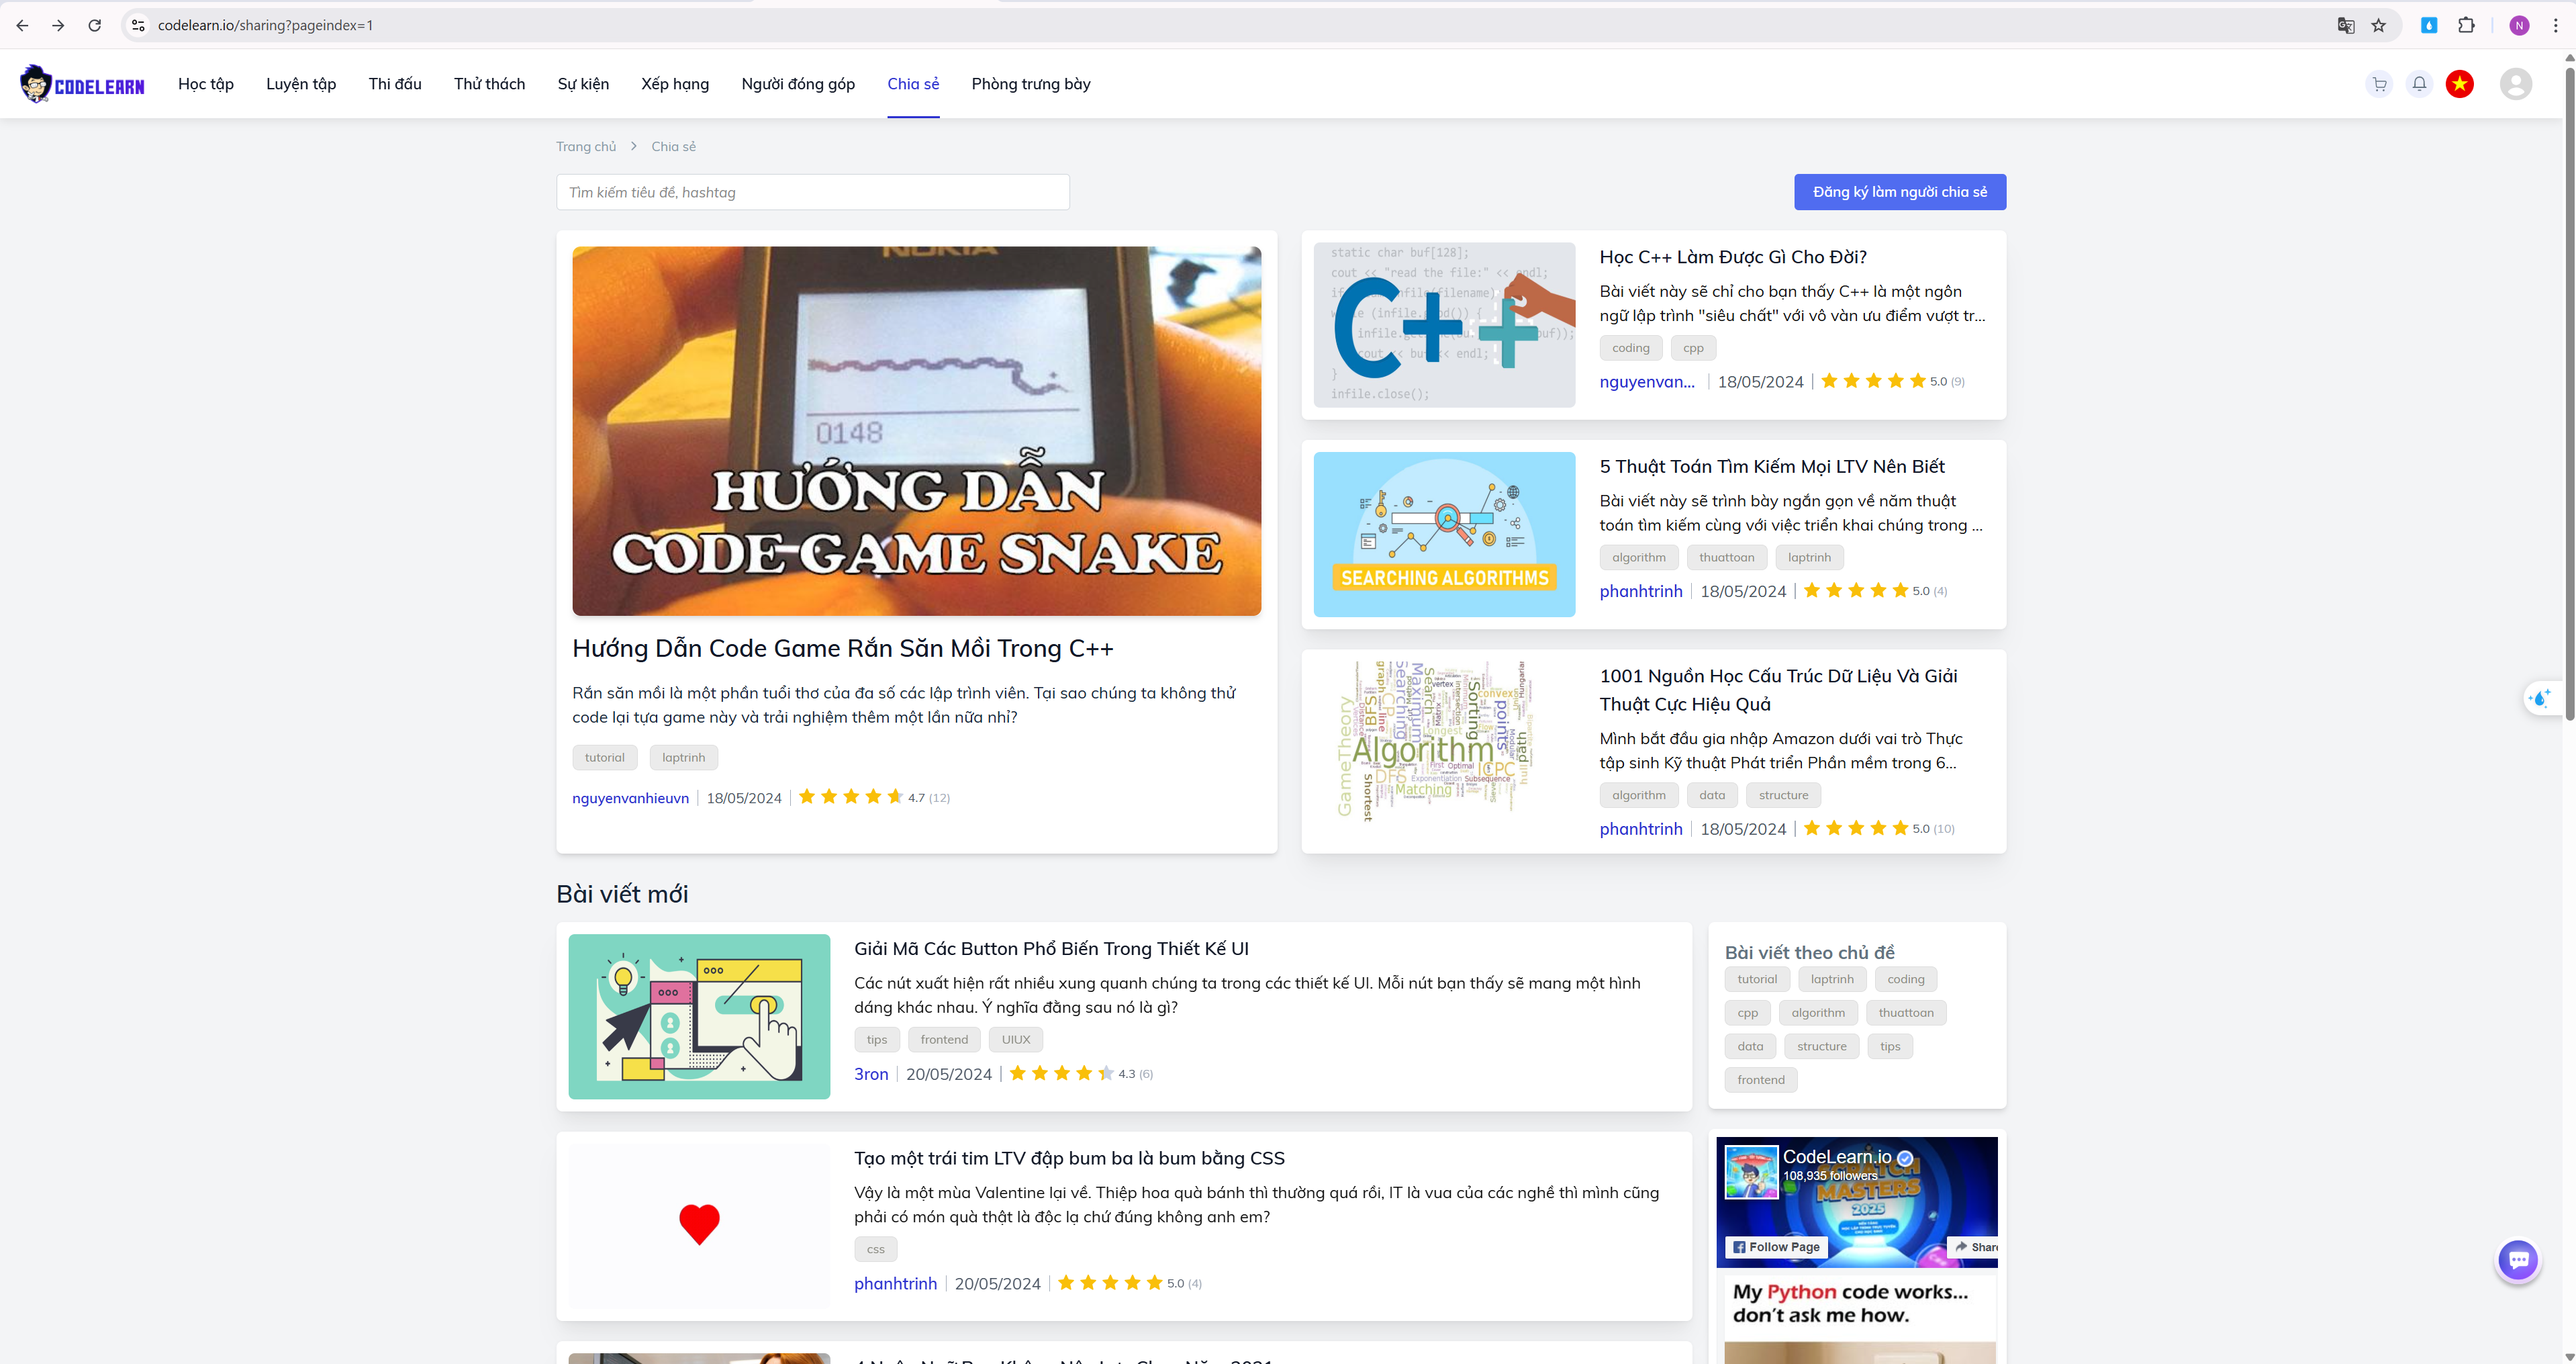
\includegraphics[width=1\linewidth]{picture/minh_chung_6.png}
    \caption{Thông tin về các bài chia sẻ}
\end{figure}

\begin{figure}[!htp]
    \centering
    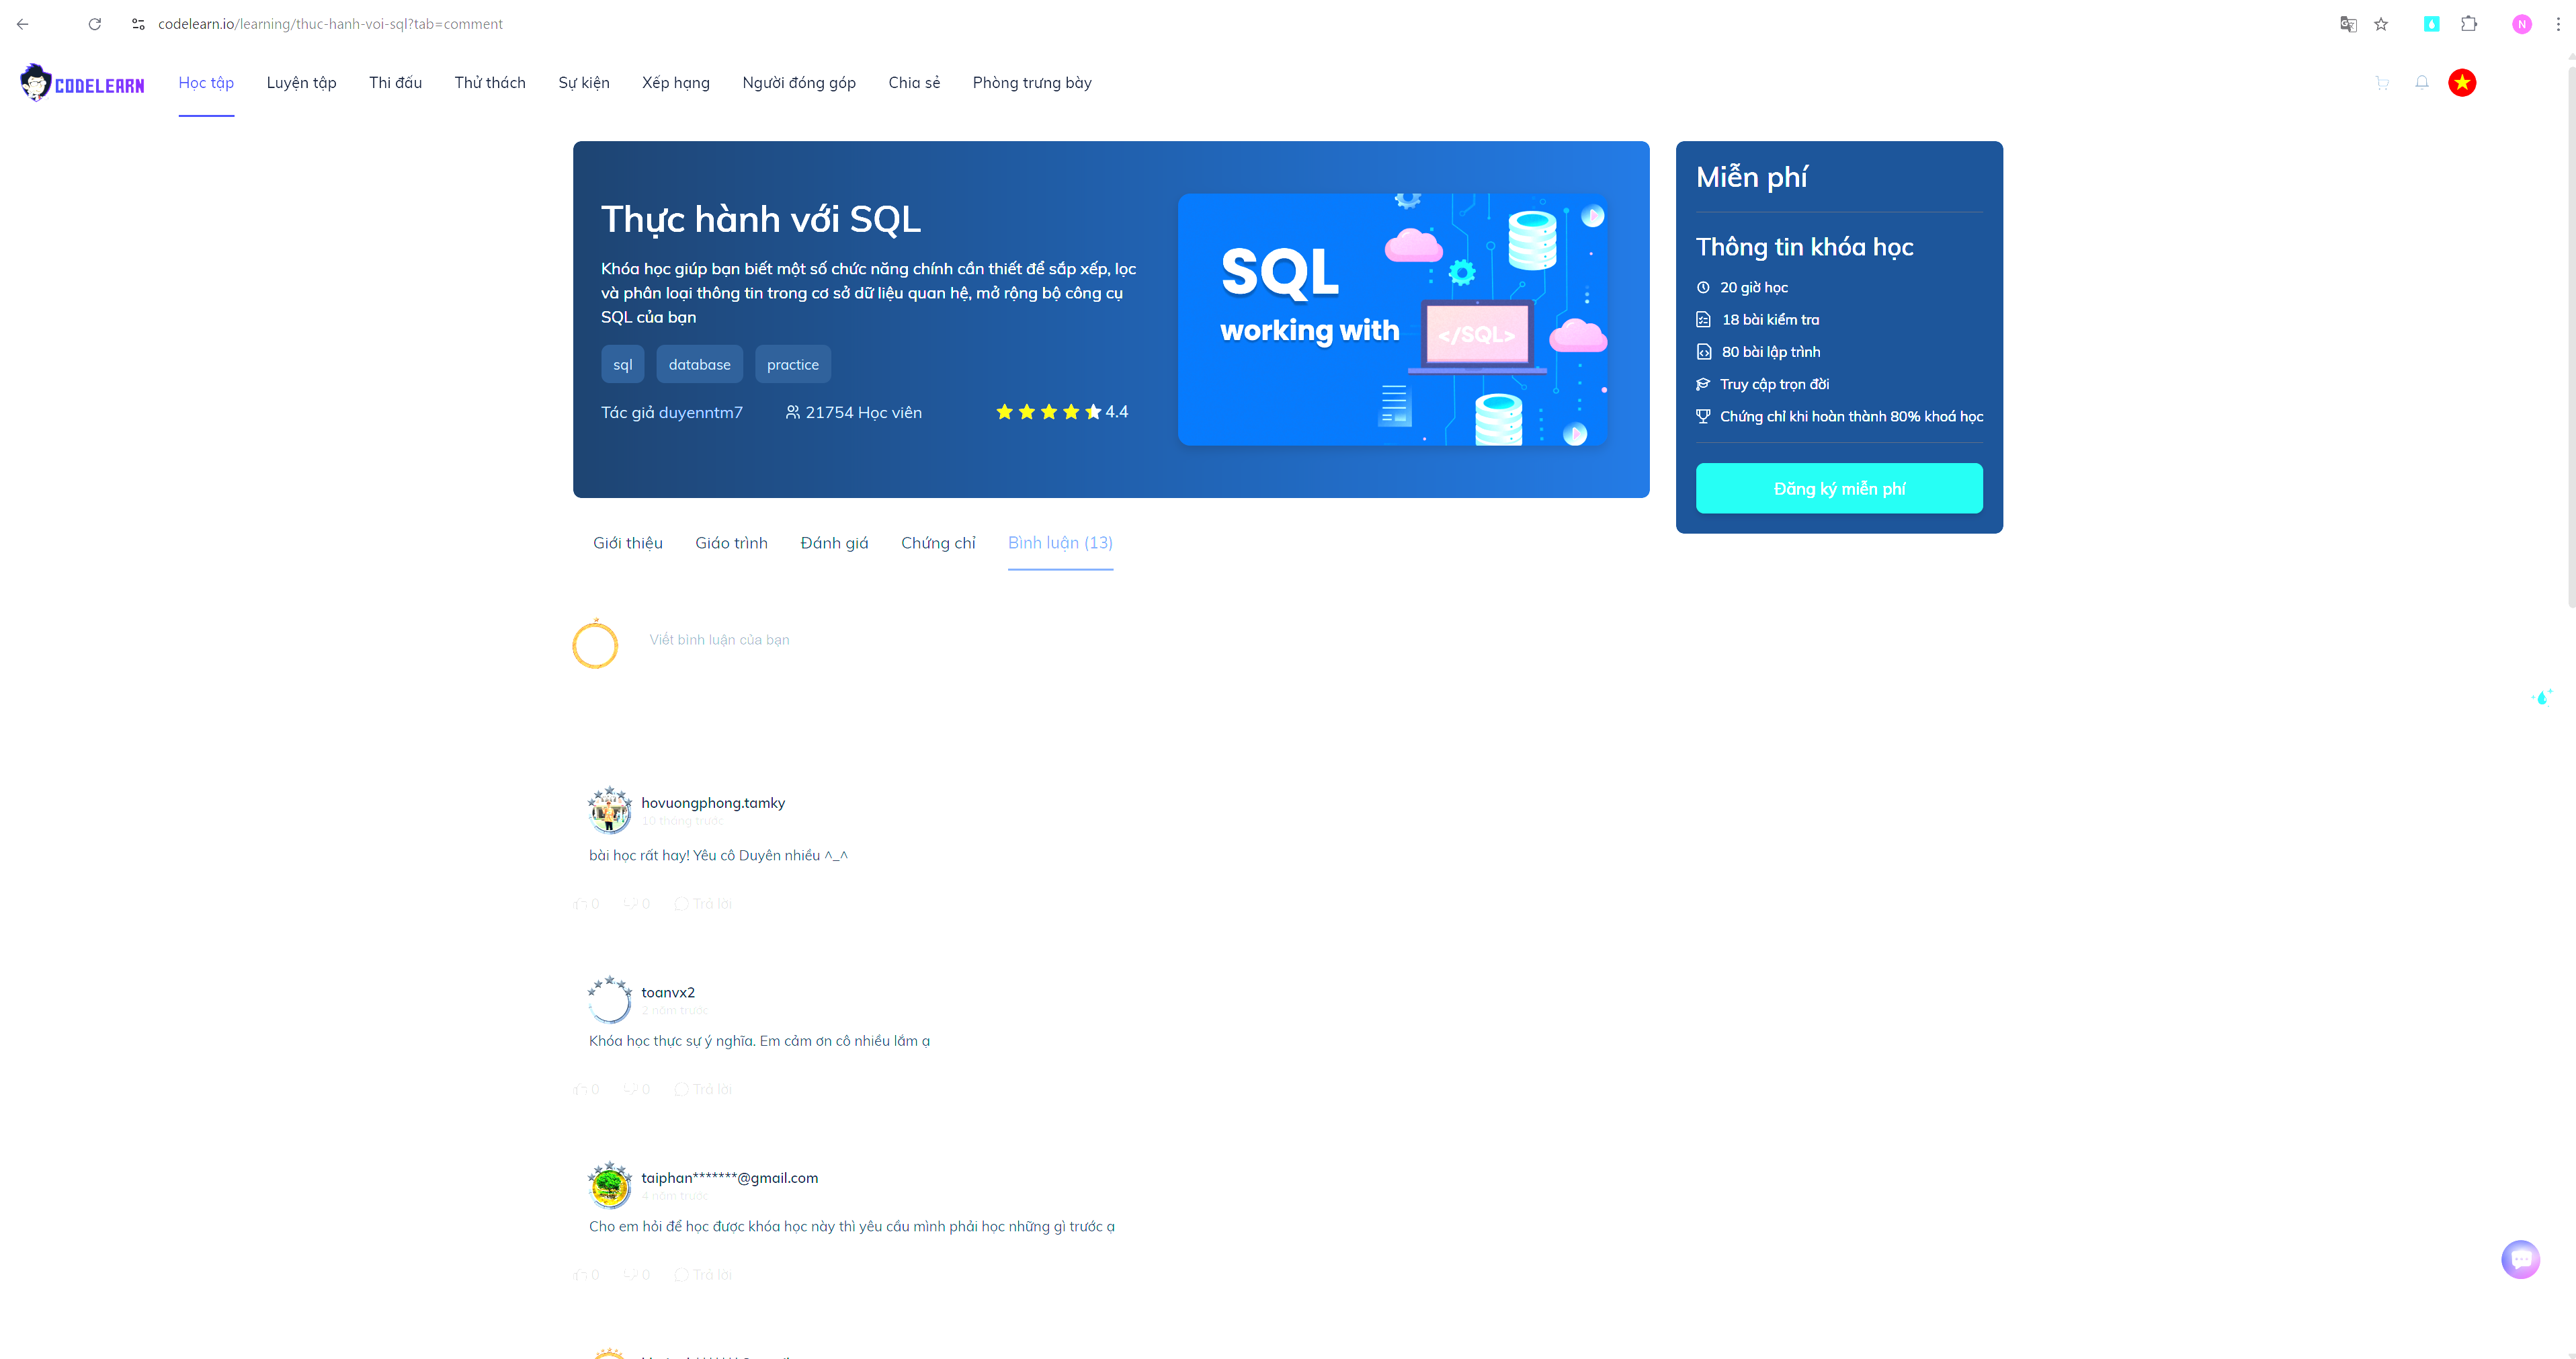
\includegraphics[width=1\linewidth]{picture/minh_chung_5.png}
    \caption{Thông tin về bình luận, đánh giá}
\end{figure}